%%%%%%%%%%%%%%%%%%%%%%%%%%%%%%%%%%%
% RSC article draft — Gamut Symmetry / Donor-Receiver Flip
% Based on RSC journal template (Royal Society of Chemistry 2016)
%%%%%%%%%%%%%%%%%%%%%%%%%%%%%%%%%%%

\documentclass[twoside,twocolumn,9pt]{article}
\usepackage{extsizes}
\usepackage[super,sort&compress,comma]{natbib}
\usepackage[version=3]{mhchem}
\usepackage[left=1.5cm,right=1.5cm,top=1.785cm,bottom=2.0cm]{geometry}
\usepackage{balance}
\usepackage{mathptmx}
\usepackage{sectsty}
\usepackage{graphicx}
\usepackage{lastpage}
\usepackage[format=plain,justification=justified,singlelinecheck=false,font={stretch=1.125,small,sf},labelfont=bf,labelsep=space]{caption}
\usepackage{float}
\usepackage{dblfloatfix}
\usepackage{fancyhdr}
\usepackage{fnpos}
\usepackage[english]{babel}
\addto{\captionsenglish}{\renewcommand{\refname}{Notes and references}}
\usepackage{array}
\usepackage{droidsans}
\usepackage{charter}
\usepackage[T1]{fontenc}
\usepackage[usenames,dvipsnames]{xcolor}
\usepackage{setspace}
\usepackage[compact]{titlesec}
\usepackage{hyperref}
\usepackage{orcidlink}
\usepackage{amsmath}
\usepackage{amssymb}
\usepackage{booktabs}
\usepackage{epstopdf}

\definecolor{cream}{RGB}{222,217,201}
\newcommand{\figureplaceholder}[2]{%
  \fbox{%
    \parbox[c][#2][c]{0.95\linewidth}{%
      \centering
      \textbf{Figure placeholder}\\[0.5ex]
      #1
    }%
  }%
}

\begin{document}
\pagestyle{fancy}
\thispagestyle{plain}
\fancypagestyle{plain}{\renewcommand{\headrulewidth}{0pt}}

\makeFNbottom
\makeatletter
\renewcommand\LARGE{\@setfontsize\LARGE{15pt}{17}}
\renewcommand\Large{\@setfontsize\Large{12pt}{14}}
\renewcommand\large{\@setfontsize\large{10pt}{12}}
\renewcommand\footnotesize{\@setfontsize\footnotesize{7pt}{10}}
\renewcommand\@biblabel[1]{#1}
\renewcommand\@makefntext[1]{\noindent\makebox[0pt][r]{\@thefnmark\,}#1}
\makeatother

\renewcommand{\thefootnote}{\fnsymbol{footnote}}
\renewcommand\footnoterule{\vspace*{1pt}\color{cream}\hrule width 3.5in height 0.4pt \color{black}\vspace*{5pt}}
\renewcommand{\figurename}{\small{Fig.}~}
\sectionfont{\sffamily\Large}
\subsectionfont{\normalsize}
\subsubsectionfont{\bf}
\setstretch{1.125}
\setlength{\skip\footins}{0.8cm}
\setlength{\footnotesep}{0.25cm}
\setlength{\jot}{10pt}
\titlespacing*{\section}{0pt}{4pt}{4pt}
\titlespacing*{\subsection}{0pt}{15pt}{1pt}
\fancyfoot{}
\fancyfoot[LO,RE]{\vspace{-7.1pt}
\includegraphics[height=9pt]{head_foot/LF}}
\fancyfoot[CO]{\vspace{-7.1pt}\hspace{13.2cm}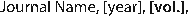
\includegraphics{head_foot/RF}}
\fancyfoot[CE]{\vspace{-7.2pt}\hspace{-14.2cm}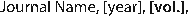
\includegraphics{head_foot/RF}}
\fancyfoot[RO]{\footnotesize{\sffamily{1--\pageref{LastPage} ~\textbar\hspace{2pt}\thepage}}}
\fancyfoot[LE]{\footnotesize{\sffamily{\thepage~\textbar\hspace{3.45cm} 1--\pageref{LastPage}}}}
\fancyhead{}
\renewcommand{\headrulewidth}{0pt}
\renewcommand{\footrulewidth}{0pt}
\setlength{\arrayrulewidth}{1pt}
\setlength{\columnsep}{6.5mm}
\setlength\bibsep{1pt}

\twocolumn[
\begin{@twocolumnfalse}
{
\includegraphics[height=30pt]{head_foot/journal_name}\hfill\raisebox{0pt}[0pt][0pt]{
\includegraphics[height=55pt]{head_foot/RSC_LOGO_CMYK}}\\[1ex]

\includegraphics[width=18.5cm]{head_foot/header_bar}}\par
\vspace{1em}
\sffamily
\begin{tabular}{m{4.5cm} p{13.5cm}}

\includegraphics{head_foot/DOI} & \noindent\LARGE{\textbf{TenKi: turning points, bias floors, and directional transfer preference in multi-fidelity autonomous materials workflows$^\dag$}} \\
\vspace{0.3cm} & \vspace{0.3cm} \\
 & \noindent\large{Kinston Ack{\"o}lf\,\orcidlink{0000-0002-5579-4878}$^{a}$ and Taylor D. Sparks\,\orcidlink{0000-0001-8020-7711}$^{*a}$} \\
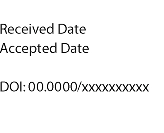
\includegraphics{head_foot/dates} & \noindent\normalsize{%
Autonomous materials workflows increasingly combine cheap, low-fidelity evaluations with expensive, high-fidelity references. A persistent question is whether scaling the number of low-fidelity measurements can always close the ranking gap to the high-fidelity reference, or whether irreducible physics differences impose a permanent floor that no amount of additional cheap data can overcome. Here we introduce TenKi (Transfer-ensemble Knowledge Inheritance, \textit{tenki}), a transfer diagnostic built on PEGKi benchmark outputs that formalises this question as a donor/receiver flip test. Using a controlled benchmark in which four physically distinct forward models and five set-operation source regions define nine competing knowledge sources -- analogous to competing computation or characterisation levels in a high-throughput materials campaign -- we show that some low-fidelity sources carry a permanent physics gap relative to the spectral reference, while others become useful at low budget. Study B, the spectral-minus-artist-RYB difference region, is the strongest unpaired donor: it achieves $\tau_{N=1}=0.619$ and $\tau_{N=10}\approx0.808$ against the high-fidelity reference. The paired Mixbox engine ($\rho = 0.990$, optimal ratio $\approx 70$) enables direct experimental validation of the allocation branches. A direct comparison of a classical control-variate branch and a hybrid ranking-fusion branch reveals a ranking-vs-estimation tradeoff: at a fixed budget of ten high-fidelity-equivalent measurements, z-score fusion achieves Kendall $\tau = 0.904$ versus $\tau = 0.821$ for the classical estimator and $\tau = 0.839$ for high-fidelity-only, because z-scoring exploits the stable ordering signal of 500 low-fidelity observations rather than estimating raw high-fidelity means. We further show that high Pearson correlation alone is not a reliable ranking-transfer diagnostic, and that set-operation source regions expose asymmetric coverage even when their names suggest shared structure. In the scheduling example developed here, this motivates separating how much budget is spent from how trustworthy a source becomes as evidence, so that source usefulness is determined by transfer structure rather than by count alone. TenKi extends the flip test to include a directional prior that encodes known scale or technique asymmetries before experiments are run, addressing cases where the conventional high-fidelity/low-fidelity direction is inverted -- such as production-scale data serving as the true reference for field performance. The results establish a practical taxonomy of donor and receiver sources and provide actionable budget-allocation guidance for autonomous formulation and discovery workflows.%
} \\
\end{tabular}
\end{@twocolumnfalse}\vspace{0.6cm}
]

\renewcommand*\rmdefault{bch}\normalfont\upshape
\rmfamily
\section*{}
\vspace{-1cm}

\footnotetext{\textit{$^{a}$~Materials Science \& Engineering, The University of Utah, 122 S. Central Campus Drive, Rm 304, Salt Lake City, Utah, USA 84112-0063. Corresponding author: Taylor D. Sparks. E-mail: taylor.sparks@utah.edu. Kinston Ack{\"o}lf publishes under this name and is also known as Kinston Wong. ORCiD: Kinston Ack{\"o}lf 0000-0002-5579-4878; Taylor D. Sparks 0000-0001-8020-7711.}}

\footnotetext{\dag~Supplementary code, benchmark data, and transfer-analysis outputs are available in the PEGKi project repository at \url{https://github.com/Sparks-Ackolf-HOLAR-Autonomous-Labs/PEGKi}. See DOI: \textit{(to be assigned)}.}


%%%MAIN TEXT%%%%

\section{Introduction}

Consider a high-throughput campaign to discover multi-principal-element alloys with superior mechanical performance.\cite{George2019HEA,Cantor2004OriginalHEA,Miracle2017HEAreview} The team has two evaluation pipelines. The first is a computational proxy: rapid first-principles calculations predict formation energies and elastic moduli at a cost of minutes per composition, allowing hundreds of candidate alloys to be screened each week. The second is a benchmark experiment: arc melting followed by nanoindentation measures true hardness and local modulus at a cost of several days per composition, limiting throughput to a handful of candidates. Both pipelines explore the same composition space, but they disagree systematically. The computational proxy is fast and broad, yet its physics model does not capture local chemical short-range order, which governs hardness in multi-principal-element alloys far more than bulk elastic constants do.\cite{Lejaeghere2016Reproducibility,Broitman2017HardnessOverview} The campaign leader faces a decision: if she runs more computational screenings -- increasing the statistical ensemble over many random supercell configurations -- does the agreement with nanoindentation improve without bound, or is there a permanent floor set by the gap in the underlying physics?

That floor, if it exists, has a further spatial dependence. Near-equiatomic compositions tend to be single-phase solid solutions, and both the computational proxy and the experiment tend to agree on their relative ranking. Off-equiatomic and multi-phase compositions occupy a different region of the accessible design space: the experiment captures precipitation-hardening contributions and grain-boundary effects that the ideal-crystal computation cannot represent, so the ranking from the two sources diverges precisely in the region that is most scientifically interesting. The campaign leader's decision about how to allocate budget between cheap and expensive evaluations therefore depends not only on the correlation between sources but also on \emph{which region of composition space} the measurements cover.

The same structure appears across many materials workflows. A fast surrogate model trained in one processing window fails once the recipe moves outside its calibration basis.\cite{Pilania2016MultiFidelityCoKriging,Tran2020MFGP} A simulation-assisted closed-loop campaign must decide whether the simulator, a historical archive, or an empirical heuristic should seed the initial prior.\cite{Gongora2021SimulationTransfer} A networked autonomous laboratory needs to know which remote source to trust before accepting its policy ranking as a guide for local experiments.\cite{Yoshida2025NetworkedAutonomous} In each case the core question is the same: is the cheap source genuinely informative about the expensive reference, and if so, at what cost and in which region of design space?

Multi-fidelity methods offer a principled framework for combining cheap and expensive information sources.\cite{Peherstorfer2018SurveyMF,KennedyOHagan2000CoKriging,Forrester2007MultiFidelityOpt,Pilania2016MultiFidelityCoKriging,Tran2020MFGP} The key quantity is the Pearson correlation $\rho$ between outcomes from the cheap and expensive evaluators across a shared set of candidates. When $\rho$ is high, a multi-fidelity control variate estimator allows the cheap source to dramatically reduce the variance of expensive estimates, and an optimal acquisition ratio $n_\mathrm{LF}/n_\mathrm{HF}$ can be derived in closed form.\cite{Peherstorfer2018SurveyMF,KennedyOHagan2000CoKriging} When $\rho$ is low, or when the cheap source carries a systematic physics bias rather than random error, no amount of additional cheap data can close the gap. The cheap source is then not a useful ``frugal twin'' for the expensive reference; it is a structurally different measurement operating under different assumptions.\cite{Lo2024FrugalTwin,Baird2023CLSLabLight}

Critically, $\rho$ alone is not always the right diagnostic. A cheap source may have a high $\rho$ in regions of design space where both sources agree, yet be systematically wrong -- inducing a biased ranking -- in the regions that matter most. Whether the gap is permanent or merely a sampling artefact, and whether it depends on which region of design space is sampled, requires a different test: a scan over measurement budget $N$ to determine whether the cheap source's ranking quality approaches the expensive reference's ceiling or saturates short of it. In the scheduling view used later in this paper, we therefore separate \emph{raw fidelity} (how much experimental or computational budget is spent) from \emph{transfer usefulness} (how much confidence that source deserves after accounting for ranking agreement, score-space transferability, bias floor, and donor stability).

Here we introduce that test as the \emph{donor/receiver flip diagnostic}. We call a source a \emph{donor} if it provides a better ranking signal than a comparison source at a given budget, and a \emph{receiver} if it provides less information than it receives. The flip question is: if a receiver source scales its budget from one measurement to $N$, does it ever surpass the donor at $N=1$? In the \emph{external} scenario, where the reference is a fixed high-fidelity ground truth, the answer determines whether the gap is a permanent physics ceiling or a sampling artefact. In the \emph{mutual} scenario, where two sources compare directly without a shared external reference, the answer is always yes at some finite $N^*$, because both sides converge to the same shared ceiling by symmetry of the ranking metric.

We demonstrate the framework using a controlled colour-formulation benchmark developed within the PyroEnGarde--Kintsugi (PEGKi) project.\cite{Ackolf2025PEGKi} PEGKi provides the matched-target databases, policy evaluations, and broader source-transfer context. The specific diagnostic introduced here is called \textbf{TenKi} (\textbf{T}ransfer-\textbf{en}semble \textbf{K}nowledge \textbf{I}nheritance, \textit{tenki}), named for the Japanese \textit{tenki}, meaning ``turning point'' or ``pivotal moment.'' In the donor/receiver context, the turning point is precisely the budget $N^*$ at which a receiver source, scaled by the number of measurements, crosses the threshold to become a donor. The \textit{Ki} carries the Kintsugi lineage from PEGKi: just as Kintsugi repairs broken ceramics with gold lacquer -- transforming damage into something more beautiful -- TenKi identifies the conditions under which an initially weak source can be elevated to a useful prior. TenKi is built on PEGKi data and extends PEGKi with a budgeted ranking diagnostic; it is not a separate framework.

Colour mixing is used here not as the target application but as a compact, chemically interpretable analogue of the alloy-screening problem described above: multiple forward models map the same nominal input (formulation coordinates) to different output regions (accessible colour gamuts), just as different computation levels map the same composition to different predicted properties. The controlled setting allows the donor/receiver structure, the bias floor, and the MFMC ratio to be characterised cleanly before TenKi is applied to noisier real materials systems.\cite{Ginsburg2023ExploringBenchmarks,Lo2024FrugalTwin,Ackolf2025PEGKi}

The core question this paper addresses is: \textit{when does low-fidelity data actually help, and when is it blocked by irreducible bias?} This question has three parts. First, what is the structure of the transfer hierarchy -- which sources are donors, which are receivers, and which carry permanent physics gaps that no amount of additional data can close? Second, how should a fixed budget be allocated across sources: does concentrating on the single highest-quality source outperform spreading budget across diverse but weaker sources? Third, when a paired low-fidelity source is available, which branch of multi-fidelity allocation -- classical control-variate estimation or hybrid ranking-fusion -- better serves ranking-only decisions versus absolute-performance decisions, and why?

The contribution should be understood at the diagnostic level. TenKi is not a new multi-fidelity estimator or a replacement for classical MFMC theory. Its novelty is a transfer diagnostic for ranking under budget. Concretely, TenKi provides four things:
\begin{enumerate}
\item \textbf{Bias-floor diagnostic}: estimates whether a source's ranking-transfer error is reducible by more samples (variance-limited) or bounded by a permanent structural ceiling (bias-limited).
\item \textbf{Donor/receiver flip test}: measures the budget $N^*$ at which a weaker source accumulates enough evidence to become a reliable donor.
\item \textbf{Paired/unpaired allocation rule}: distinguishes classical control-variate estimation (requires paired targets, valid for absolute-performance decisions) from hybrid ranking fusion (valid for any source, ranking decisions only).
\item \textbf{Negative controls}: shows that high Pearson correlation and naive source aggregation can both fail as ranking-transfer diagnostics, motivating the $\tau(N)$ convergence curve as the correct prior diagnostic.
\end{enumerate}
TenKi does not claim to provide a general proof of transfer across all materials domains, a one-shot reliable donor at $N=1$, or a new scheduling algorithm (the async optimizer in Experiment 13 is a demonstration, not a core claim). TenKi is the budgeted source-selection layer of PEGKi: PEGKi identifies directional transfer structure across modalities, while TenKi estimates the sampling budget and bias floor associated with each candidate donor source.

\begin{figure}[h]
    \centering
    \figureplaceholder{%
        Schematic of the donor/receiver flip problem. Four pigment-mixing modalities define different regions of accessible colour space. A ``donor'' source provides ranking information that a ``receiver'' cannot match at the same budget. The flip question asks whether scaling the receiver's budget ever reverses the relationship.%
    }{5.0cm}
    \caption{The donor/receiver flip diagnostic. Multiple source modalities occupy overlapping but asymmetric regions of the accessible response space (top), analogous to different computation or measurement levels covering different regions of composition space in an alloy-screening campaign. The ranking quality $\tau(N)$ of each source vs. the high-fidelity reference increases with budget $N$ but saturates at a physics ceiling that may fall short of 1.0 even as $N \to \infty$ (bottom). A permanent gap identifies a receiver source that cannot become a donor regardless of budget; a finite $N^*$ identifies a flippable source.}
    \label{fig:concept}
\end{figure}

The specific aims of this work are threefold. First, to determine the transfer structure of the source hierarchy: which sources are donors, which are receivers, and which carry permanent external gaps that no amount of additional budget can close. Second, to determine how a fixed budget should be allocated across candidate low-fidelity sources: whether concentration on the best donor outperforms spreading budget across diverse but weaker sources. Third, to determine when paired multi-fidelity allocation helps ranking decisions and when it only helps scalar estimation, by comparing a classical control-variate branch against a hybrid ranking-fusion branch. The coverage-geometry analysis and the derived study databases provide the structural explanation for these outcomes. Figure~\ref{fig:concept} frames the central diagnostic.

\section{Experimental}

\subsection{Benchmark rationale and modality definitions}

We use inverse colour matching as a compact but physically interpretable analogue of a general materials formulation problem. The same four-component composition vector $(R, Y, B, W)$ with $R + Y + B + W = 100$ is evaluated under four different pigment-mixing modalities that each embed different physics, calibration data, and accessible gamut regions. Identical nominal inputs do not produce identical colour outputs because each modality maps the same formulation coordinates through a different forward model. This is precisely the kind of context shift that recurs when a synthesis recipe moves between a first-principles calculation, a calibrated process model, and a measured characterisation regime.

The four base modalities are: a Beer--Lambert dye-absorption model (BL), which uses spectral transmittance under CIE D65 illumination;\cite{Kubelka1931} a Mixbox surrogate pigment model (MB);\cite{Sochorova2021} a Kubelka--Munk model (KM) anchored to measured oil-pigment $K/S$ spectra;\cite{Wiersma2025Hyperspectral} and an artist RYB mixing model (RYB).\cite{Gossett2004RYB} In the context of the flip test, the BL modality is the high-fidelity (HF) spectral reference because it captures physical transmittance spectra through real dye absorption coefficients. The remaining three single-modality sources and five set-operation source regions serve as candidate low-fidelity (LF) sources whose correlation with and independence from the spectral reference are characterised here.

Each source modality $K_j$ defines its own forward map
\[
f_j : \mathcal{X} \rightarrow \mathcal{Y}_j
\]
from the shared composition space $\mathcal{X}$ to a modality-specific colour response $\mathcal{Y}_j$. The inverse-design task for a target colour $y^*$ is
\[
x^*_j \in \arg\min_{x \in \mathcal{X}} d\!\left(f_j(x),\, y^*\right),
\]
with the same nominal composition variables and the same target used across all modalities but with a different contextual map $f_j$ in each case. The accessible gamut of each modality is therefore different, and regions of colour space are covered asymmetrically.

\subsection{Set-operation study databases}

\begin{figure*}[!t]
    \centering
    \figureplaceholder{%
        Four-panel Venn geometry of modality gamuts. Panels show: (left) pairwise overlap volumes for all six engine pairs visualised as a matrix of Jaccard indices; (centre-left) asymmetry indices for each pair; (centre-right) three-way and four-way intersection volumes; (right) schematic of the nine source databases placed within the overall Venn diagram.%
    }{5.5cm}
    \caption{Venn geometry of the four base modalities at voxel resolution 40. Pairwise Jaccard indices [\textsc{placeholder}: run experiment 01], asymmetry indices [\textsc{placeholder}], and multi-engine intersection volumes [\textsc{placeholder}] are shown. The five set-operation databases occupy the MB+RYB overlap and the BL$-$RYB, RYB$-$BL, KM$-$MB, and MB$-$KM difference regions. A key observation is that intersection regions are not geometrically centred: the MB+RYB intersection region has mean RGB far from neutral grey $(128,128,128)$, demonstrating that set-theoretic intersection does not imply symmetry.}
    \label{fig:venn_geometry}
\end{figure*}

From the four base modalities we construct five set-operation study databases on the modality gamuts (Table~\ref{tab:study_matrix}). Study A is drawn from the MB+RYB intersection region: colours that both Mixbox and RYB reproduce within a defined agreement threshold. Study B and Study B-reverse are drawn from the BL$-$RYB and RYB$-$BL difference regions. Study C and Study C-reverse are drawn from the KM$-$MB and MB$-$KM difference regions.

These databases span the PEGKi set-operation taxonomy: Study A is an overlap dataset (type $K_{\mathrm{H\_OVERLAP}}$), while the directional difference regions probe transfer and exclusion asymmetries. The gamut geometry underlying these databases is characterised in Experiment 01 (Fig.~\ref{fig:venn_geometry}) and the resulting directed transfer structure is established in Experiment 02.

\begin{table}[h]
\small
\caption{\ Study database matrix. BL = Beer--Lambert; MB = Mixbox; KM = Kubelka--Munk; RYB = artist RYB.}
\label{tab:study_matrix}
\begin{tabular*}{0.48\textwidth}{@{\extracolsep{\fill}}llll}
\hline
\textbf{Label} & \textbf{Set operation} & \textbf{KS type} & \textbf{Bias floor} \\
\hline
Study A & MB $\cap$ RYB & $K_{\mathrm{H\_OVERLAP}}$ & 0.167 \\
Study B & BL $-$ RYB   & $K_T$                     & 0.167 \\
Study B-rev. & RYB $-$ BL & $K_T$                  & 0.167 \\
Study C & KM $-$ MB     & $K_E$                     & 0.278 \\
Study C-rev. & MB $-$ KM & $K_E$                   & 0.167 \\
\hline
\end{tabular*}
\end{table}

\subsection{Ranking quality metric and flip test protocol}

The primary ranking-quality metric is Kendall's $\tau$\cite{Kendall1938TauCorrelation} between the policy ranking produced by source $i$ using $N$ experiments and the policy ranking produced by the full spectral reference:
\[
\tau_{ij}(N) = \mathrm{Kendall\text{-}}\tau\!\bigl(\hat{r}_i(N),\, r_j^{(\infty)}\bigr),
\]
where $\hat{r}_i(N)$ is the ranking produced by averaging $N$ independently drawn experiment scores for source $i$, and $r_j^{(\infty)}$ is the full-data ranking for reference $j$. The \emph{physics ceiling} of source $i$ relative to spectral is
\[
\mathrm{ceiling}(i) = \lim_{N \to \infty} \tau_{i,\,\mathrm{spectral}}(N),
\]
estimated empirically as $\tau_{i,\,\mathrm{spectral}}$ at full $N$. The \emph{bias floor} is $1 - \mathrm{ceiling}(i)$.

The \emph{external flip test} asks whether source $A$, with budget $N$, can surpass source $B$ at $N=1$ as a proxy for the spectral reference:
\[
N^*_{\mathrm{ext}}(A \to B) = \min\!\left\{ N : \tau_{A,\,\mathrm{spectral}}(N) > \tau_{B,\,\mathrm{spectral}}(1) + \epsilon \right\},
\]
where $\epsilon = 0.02$ is a significance threshold. If $\mathrm{ceiling}(A) < \mathrm{ceiling}(B)$, the external flip is impossible at any $N$ (a permanent gap). The \emph{mutual flip test} uses the shared ceiling: because Kendall's $\tau$ is symmetric, $\tau_{AB}(\infty) = \tau_{BA}(\infty)$ always, so a mutual flip is always possible at some finite $N^*_{\mathrm{mut}}$.

Bootstrap resampling ($n_\mathrm{bootstrap} = 300$) at each budget level $N \in \{1, 2, 3, 5, 8, 10, 15, 20, 30, 50, 100, 200, 500, 1000\}$ provides uncertainty estimates on $\tau(N)$ curves. The frugal-twin convergence analysis (Experiment 07) uses $N \in \{1, \ldots, 100\}$; the canonical flip-test run (Experiment 03) uses $N \in \{1, \ldots, 1000\}$. Directed transfer matrices are computed from the $N = 1$ asymmetry $A[i,j] = \tau_{ij}(1) - \tau_{ji}(1)$, which identifies which source is the donor and which is the receiver in a single-experiment comparison.

\subsection{Multi-fidelity acquisition protocol}

For each candidate LF source, we estimate the Pearson correlation $\rho$ between per-policy performance scores under the LF source and the HF spectral reference across the shared policy set. The multi-fidelity Monte Carlo (MFMC) optimal acquisition ratio is then\cite{Peherstorfer2018SurveyMF}
\[
\frac{n_\mathrm{LF}}{n_\mathrm{HF}} = \sqrt{r} \cdot \frac{|\rho|}{\sqrt{1 - \rho^2}},
\]
where $r = \mathrm{cost}(\mathrm{HF}) / \mathrm{cost}(\mathrm{LF})$ is the cost ratio. We report results at $r = 100$ as a representative ratio appropriate for spectrophotometer-versus-colorimeter comparisons in formulation laboratories. The cost-efficiency curve compares the ranking quality $\tau$ achieved by a mixed HF+LF campaign as a function of total budget expressed in HF-equivalents, against a HF-only campaign of the same budget.

For the async optimizer extension, this MFMC ratio is treated as a \emph{raw-budget} rule rather than as a full definition of fidelity. The scheduler still spends explicit budget units such as number of experiments or rounds. However, the optimizer scores each $(\text{source}, \text{raw fidelity})$ state using a transfer-usefulness score that combines Kendall $\tau$, Pearson $\rho$, the estimated bias floor, and donor/receiver stability. In other words, nominal budget and source trust are separated: more measurements increase raw fidelity, but they count as genuinely ``better evidence'' for routing only insofar as they improve the inferred transfer state.

\subsection{Directional transfer preference and scale-exclusive phenomena}

The flip test and MFMC ratio both treat the high-fidelity source as a fixed reference and ask how cheaply it can be approximated. That framing implicitly assumes that information should flow from cheap to expensive -- from LF to HF calibration. However, this direction is not always correct. Some phenomena are \emph{scale-exclusive}: they are only observable at one scale or one modality, and the ``expensive'' measurement is not always the one conducted under idealised laboratory conditions.

Consider a few representative reversals. In fatigue life assessment of structural alloys, laboratory samples are small, defect-free, and loaded under controlled cyclic stress. Production-scale components contain weld zones, surface oxidation, and residual stresses from manufacturing; the statistical spread in fatigue life at production scale cannot be inferred from laboratory samples regardless of how many laboratory tests are run. The production (fab) measurement is the higher-fidelity reference for field failure prediction, and knowledge should flow from fab to lab rather than the reverse. Similarly, in thin-film photovoltaics, module-level degradation mechanisms -- edge delamination, interconnect corrosion, thermomechanical stress at cell boundaries -- are invisible in small-area laboratory cells. The module measurement is the ground truth for bankability prediction. In both cases, treating the laboratory measurement as the HF reference and the production measurement as the LF proxy inverts the true information hierarchy.

A second class of reversals arises from \emph{technique-exclusive} phenomena. Short-range chemical order in multi-principal-element alloys is only observable by atom-probe tomography or diffuse neutron scattering; bulk hardness averages over millions of local environments and cannot rank compositions by their short-range ordering tendency no matter how many measurements are taken. The technique that costs more per measurement is not always the reference; the technique that has access to the mechanistically relevant variable is.

To accommodate these cases within the donor/receiver framework, we propose augmenting the transfer score with a physics-informed directional prior $\pi(K_s \to K_t) \in [-1, +1]$:
\begin{equation}
\Delta'(K_s \to K_t) = \lambda_\pi \, \pi(K_s \to K_t) + \lambda_\sigma \, \sigma(K_s, K_t) + \lambda_\rho \, \rho(K_s, K_t) - \lambda_\omega \, \omega(K_s, K_t),
\label{eq:delta_prime}
\end{equation}
where $\pi > 0$ encodes the belief that the source $K_s$ is the natural donor for target $K_t$ (e.g., fab is the reference for field performance), $\pi < 0$ penalises the transfer direction as physically implausible, and $\pi = 0$ recovers the empirical-only transfer score. The weight $\lambda_\pi$ controls how strongly the prior overrides or augments the empirical signal. In the limit $\lambda_\pi \to 0$, all information about direction comes from the observed $\tau$ curves. In the limit $\lambda_\pi \gg \lambda_\rho$, the physics prior dominates and the framework encodes a known asymmetry before any experiment is run.

The MFMC ratio already handles the cost-direction reversal naturally. If the fab measurement is the HF reference and the lab measurement is the cheaper LF source, one simply assigns $r = \mathrm{cost}(\mathrm{fab}) / \mathrm{cost}(\mathrm{lab})$. If this ratio is less than one (lab measurements are more expensive per unit of information than fab measurements), the MFMC ratio decreases accordingly. The framework does not enforce a direction; it takes whatever source is designated as reference and asks how efficiently the other source can approximate it. The directional prior $\pi$ makes that designation explicit and principled rather than leaving it implicit in the labeling convention.

In the current benchmark, the BL spectral source is the natural HF reference by physical construction: it measures full transmittance spectra and uses real dye absorption coefficients, while the other modalities use simplified or surrogate physics. The $\pi$ prior is therefore unnecessary here, and we set $\lambda_\pi = 0$ throughout. The extension to directional-prior-weighted transfer is reserved for settings where the reference direction is not determined by model fidelity alone.

\section{Results and discussion}

\subsection{How to read the results}

The results answer three supporting questions that together address when low-fidelity data helps and when it is blocked by irreducible bias. The structural question (Q1) characterises the transfer hierarchy: which sources are donors, which are receivers, and which carry permanent physics gaps. The empirical question (Q2) addresses fixed-budget allocation: does concentrating on the single best source outperform spreading budget across diverse sources? The engineering question (Q3) examines multi-fidelity branch selection: classical control-variate estimation versus hybrid ranking-fusion, and when each wins. Q1 is answered by Experiments 01--04; Q2 by Experiments 05--07; Q3 by Experiment 08. The synthesis in Table~\ref{tab:source_taxonomy} and the six-step decision rule in the Synthesis subsection consolidate all three.

\subsection{Q1 -- Structural: gamut geometry and donor/receiver hierarchy}

\noindent\textit{This section summarises the structural results already established by Experiments 01--04. The figures remain placeholders in the current draft, but the numerical statements below reflect the current TenKi result bundle rather than a future planned analysis.}

\begin{figure*}[!t]
    \centering
    \figureplaceholder{%
        Four-panel Venn geometry of modality gamuts. Panels show: (left) pairwise Jaccard indices; (centre-left) asymmetry indices; (centre-right) three-way and four-way intersection volumes; (right) schematic of the nine source databases placed within the overall Venn diagram.%
    }{5.5cm}
    \caption{Venn geometry of the four base modalities at voxel resolution 40. The current draft uses a placeholder figure; the quantitative interpretation is that the five set-operation databases occupy the MB+RYB overlap and the BL$-$RYB, RYB$-$BL, KM$-$MB, and MB$-$KM difference regions.}
    \label{fig:venn_geometry}
\end{figure*}

\begin{figure}[h]
    \centering
    \figureplaceholder{%
        Directed transfer matrix at $N = 1$ across all nine sources. Colour encodes $\tau_{ij}(1) - \tau_{ji}(1)$: positive (red) means row is donor, negative (blue) means row is receiver. Diagonal is undefined.%
    }{4.5cm}
    \caption{Directed transfer matrix $A[i,j] = \tau_{ij}(1) - \tau_{ji}(1)$ at $N=1$. The current draft uses a placeholder figure; the established qualitative result is a largely transitive hierarchy with spectral at the apex.}
    \label{fig:transfer_matrix}
\end{figure}

The Venn geometry analysis (Experiment 01, Fig.~\ref{fig:venn_geometry}) maps the pairwise Jaccard overlaps, volume asymmetry indices, and multi-engine intersection volumes for all four source modalities. A key result is that the MB+RYB intersection region is not geometrically centred: its mean RGB centroid is approximately $(189, 127, 121)$, well displaced from the neutral grey point $(128, 128, 128)$ and biased toward warm, desaturated red--orange hues. Intersection is a set-theoretic operation, not a symmetrisation. The intersection selects the agreement region of two models that are both biased in the same direction, so the resulting dataset inherits both biases.

The Experiment 05 symmetry scoring analysis already confirms that the three study databases form a nearly disjoint partition: pairwise overlap is negligible, and K=3 databases achieve knowledge-space balance with a perfect score of $1.0$. Full engine-permutation symmetry across all four modalities would require K=15 databases (one per non-empty Venn region); only three are currently populated.

The directed transfer matrix (Experiment 02, Fig.~\ref{fig:transfer_matrix}) quantifies which sources are donors and which are receivers at single-experiment budget $N=1$. The flip-test ceiling evidence establishes the external donor hierarchy: spectral is the apex donor, Study B ($\tau_{N=10} = 0.808$, $\tau_{N=1} = 0.619$, bias floor $= 0.167$) is the best LF proxy, and Study A ($\tau_{N=1} = 0.221$, same ceiling as Study B) is the worst despite its intersection label. Study A and Study B share the same full-data ceiling ($\tau = 0.833$); Study B's advantage is a much higher single-experiment tau and correspondingly faster convergence to that ceiling. Notably, at $N=1$ only Study B and Mixbox qualify as donors ($\tau > 0.5$); RYB, despite having the highest ceiling, is a receiver at $N=1$ ($\tau_{N=1} = 0.497$) and requires roughly eight experiments to transition.

\begin{figure}[h]
    \centering
    \figureplaceholder{%
        Flip test curves for each study vs. spectral. Each panel shows $\tau(N)$ vs. $N$ for one LF source (solid) and the single-experiment $\tau$ of the spectral reference (dashed). The horizontal dashed line is the physics ceiling.%
    }{5.0cm}
    \caption{External flip test: $\tau(N)$ curves for each candidate LF source. The current draft uses a placeholder figure; the established interpretation is that Study B converges to ceiling $= 0.833$ (bias floor $= 0.167$), Study A converges to the same ceiling but far more slowly, and Study C has the lowest ceiling at $0.722$ (bias floor $= 0.278$), confirming permanent physics gaps for all three sources.}
    \label{fig:flip_test}
\end{figure}

The flip feasibility analysis (Experiments 03 and 04, Fig.~\ref{fig:flip_test}) partitions the source space into permanently gapped sources and flippable sources, and measures the mutual flip cost $N^*_\mathrm{mut}$ for each pair. The bias floors from Experiment 07 are consistent with all three study databases carrying permanent external physics gaps relative to the spectral reference. In the mutual scenario, all pairs are flippable at finite $N^*_\mathrm{mut}$ because the shared Kendall $\tau$ ceiling guarantees convergence from both sides.

\subsection{Q2 -- Empirical: source quality dominates over diversity}

\begin{figure}[h]
    \centering
    \figureplaceholder{%
        Kendall $\tau$ vs. number of robots (swarm size $N$) for all three study databases and the spectral reference itself. Shaded bands show bootstrap 95\% intervals. Horizontal dotted line at $\tau = 0.80$.%
    }{4.5cm}
    \caption{Frugal twin convergence curves. Kendall $\tau$ vs.\ swarm size $N$ for each LF source compared against the full spectral ranking ($n_\mathrm{bootstrap}=200$, $N \in \{1,\ldots,100\}$). Study B (blue) starts near $\tau_{N=1} \approx 0.61$, reaches $\tau \geq 0.80$ at approximately $N = 10$, and converges to a full-data ceiling of $0.833$ (bias floor $= 0.167$). Study A (orange) starts far lower at $N=1$ ($\tau \approx 0.2$) and converges to the \emph{same} ceiling of $0.833$, but requires far more experiments. Study C (green) has the largest permanent gap (ceiling $= 0.722$, bias floor $= 0.278$). For reference, the spectral source itself (dashed) converges to $\tau = 1.0$ by construction.}
    \label{fig:frugal_convergence}
\end{figure}

The frugal twin convergence curves (Fig.~\ref{fig:frugal_convergence}, Experiment 07) reveal a clear and practically important result: source quality dominates over diversity of source coverage at all budget levels tested. Study B reaches ranking quality $\tau \geq 0.80$ with approximately 10 experiments, a budget readily achievable in most formulation laboratories. At 100 experiments the bootstrap mean converges to $\tau \approx 0.89$ (see Table~\ref{tab:source_taxonomy} for the full-data ceiling and bias floor).

Study A, despite being drawn from the intersection region -- which might naively suggest it captures the ``common core'' most relevant to the spectral reference -- is the worst frugal proxy. It begins at $\tau = 0.221$ at $N=1$, far below Study B's $N=1$ value of $0.619$, and converges to only $0.833$ even at large $N$. The intersection region is biased toward warm, high-chroma hues where both Mixbox and RYB agree, but the spectral reference encodes the broadest gamut including the cool blues and cyans that the artist-RYB model cannot produce and therefore excludes from the intersection. The intersection dataset is thus systematically misaligned with the spectral reference's ordering.

Study C has the largest permanent gap (bias floor $= 0.278$, ceiling $= 0.722$; Table~\ref{tab:source_taxonomy}) and the lowest overall convergence trajectory. The KM$-$MB difference region captures colours specific to the measured oil-pigment model, but those colours lie in regions of colour space where the spectral reference's ranking signal is difficult to reproduce from either difference-region source.

The fixed-budget diversity test (Experiment 07, Q3 and Q3b) quantifies this precisely. In the $k$-sweep at $N_\mathrm{total} = 10$, the best single-study allocation is Study B with $\tau = 0.794$, and performance decreases monotonically as more study types are added. In the saved Q3b single-vs-all comparison, the script's best-single baseline is Mixbox: at $N_\mathrm{total} = 10$, Mixbox alone achieves $\tau = 0.764$ whereas spreading the same budget equally across the tested LF source pool achieves only $\tau = 0.578$, a degradation of $\Delta\tau = -0.186$. The gap narrows as budget increases (to $\Delta\tau = -0.050$ at $N_\mathrm{total} = 100$) but concentration still wins at every level tested. Diversity across KS types helps raise the floor when no single source is good enough, but once a high-quality source is available it should receive the full budget. This matches intuition from multi-source materials workflows: routing budget away from a $\rho = 0.990$-correlated source toward weaker alternatives dilutes rather than strengthens the ensemble.

\subsection{Q3 -- Engineering: optimal multi-fidelity acquisition ratio}

\begin{figure*}[!t]
    \centering
    \figureplaceholder{%
        Three panels. Left: MFMC optimal ratio curves vs.\ cost ratio $r$ for each paired LF source. Centre: cost-efficiency curves at $r=100$ comparing classical (paired CV), hybrid (z-score fusion), and HF-only branches (Mixbox LF). Right: per-policy MSE of the classical branch estimator vs.\ budget, shown on a log scale.%
    }{5.0cm}
    \caption{Multi-fidelity acquisition analysis (Experiment 08, 1000-target benchmark, $N_\mathrm{bootstrap}=500$).
    \textit{Left}: MFMC optimal LF:HF ratio at $r=100$ for each paired LF source (Mixbox $\rho=0.990$, RYB $\rho=0.986$, KM $\rho=0.973$).
    \textit{Centre}: Kendall $\tau$ vs.\ total budget $B$ for the classical control-variate branch, the hybrid ranking-fusion branch, and the HF-only baseline (Mixbox as LF, $r=100$). The hybrid branch dominates both classical and HF-only at all budget levels; the classical branch is approximately equal to HF-only.
    \textit{Right}: Per-policy MSE of the classical branch estimator of $\mu_\mathrm{HF}$ vs.\ budget, shown on a log scale. Policies with large oracle $\alpha$ (e.g.\ neural network, $\alpha=0.75$) show genuine variance reduction; policies with small $\alpha$ (e.g.\ Bayesian EI, $\alpha=0.017$) show negligible improvement over HF-only.}
    \label{fig:mfmc}
\end{figure*}

Experiment 08 separates the multi-fidelity allocation question into two distinct branches with different estimands, making the ranking-vs-estimation tradeoff explicit.

\paragraph{Classical branch.}
The classical branch implements the textbook MFMC control-variate estimator (see Supplementary Information).  For each policy $p$, it estimates the true HF mean $\mu_p = \mathbb{E}_t[\mathrm{best\_cd}(\mathrm{HF}, t, p)]$ using $n_\mathrm{HF}$ paired HF/LF target observations and $n_\mathrm{LF}$ additional LF-only observations, with an oracle control-variate coefficient $\alpha_p = \mathrm{Cov}(Y_\mathrm{HF}, Y_\mathrm{LF})/\mathrm{Var}(Y_\mathrm{LF})$ estimated from all 1004 available paired experiments.  Policies are then ranked by estimated $\hat{\mu}_p$.

Three LF sources are valid for this branch because they share target colours by experiment index with the spectral reference (generated with a common shared-targets file): Mixbox ($\rho = 0.990$), RYB ($\rho = 0.986$), and KM ($\rho = 0.973$).  The set-operation study databases were generated on different target spaces and cannot be paired.

\paragraph{Hybrid branch.}
The hybrid branch is a ranking heuristic, not a scalar estimator.  It z-scores independent HF and LF sample means across policies and fuses them as
\[
    z_\mathrm{cv}(p) = z_\mathrm{HF}(p) + \rho \cdot z_\mathrm{LF}(p),
\]
then sorts policies by $z_\mathrm{cv}$ ascending.  The estimand is Kendall $\tau$ vs.\ the full HF ranking, not $\mu_p$.  This branch is valid for any LF source, paired or unpaired.  Both branches use the same budget model ($B = n_\mathrm{HF} + n_\mathrm{LF}/r$) and the same MFMC-optimal allocation prior.

\paragraph{Empirical result.}
Using Mixbox as LF at $r = 100$, the hybrid branch achieves $\tau = 0.904$ at budget $B = 10$ (5 HF + 500 LF), versus $\tau = 0.821$ for the classical branch and $\tau = 0.839$ for HF-only.  The hybrid dominates at all budget levels by $\Delta\tau \in [0.048, 0.141]$ (Table~\ref{tab:mfmc_compare}).

\begin{table}[h]
\centering
\caption{Kendall $\tau$ comparison: classical vs.\ hybrid branch (Mixbox LF, $r=100$, $N_\mathrm{bootstrap}=500$). Budget $B$ in HF-equivalent units.}
\label{tab:mfmc_compare}
\begin{tabular}{rrrrrr}
\hline
$B$ & $n_\mathrm{HF}$ & $n_\mathrm{LF}$ & Classical $\tau$ & Hybrid $\tau$ & HF-only $\tau$ \\
\hline
2 & 1 & 100 & 0.676 & \textbf{0.800} & 0.721 \\
5 & 2 & 300 & 0.757 & \textbf{0.850} & 0.798 \\
10 & 5 & 500 & 0.821 & \textbf{0.904} & 0.839 \\
20 & 11 & 900 & 0.870 & \textbf{0.942} & 0.881 \\
50 & 29 & 2100 & 0.917 & \textbf{0.974} & 0.923 \\
100 & 58 & 4200 & 0.939 & \textbf{0.987} & 0.947 \\
\hline
\end{tabular}
\end{table}

\paragraph{Why classical loses on $\tau$.}
The oracle $\alpha_p$ values for the best-ranked policies are very small: Bayesian EI ($\alpha = 0.017$), Bayesian UCB ($\alpha = 0.058$), and simulated annealing ($\alpha = -0.008$).  A small $\alpha$ means the control-variate correction is negligible -- the classical estimator reduces to plain HF-only averaging for precisely the policies that determine the top of the ranking.  The variance reduction that MFMC theory predicts only materialises when $\alpha_p$ is large (e.g.\ neural network: $\alpha = 0.75$).

The hybrid's advantage over classical is structural: z-scoring discards absolute scale entirely, so 100--4200 LF observations with $\rho = 0.990$ identify the ordering reliably, regardless of whether the raw LF means are close to the HF means.

\paragraph{Classical wins on estimation faithfulness.}
The classical branch is the correct choice whenever the estimand is $\mu_p$ itself rather than rank order.  The MSE curves (Fig.~\ref{fig:mfmc}, right) confirm that policies with large $\alpha$ show genuine variance reduction; the estimator is unbiased by construction.  For any claim about absolute performance levels -- such as ``policy $p$ achieves a mean colour distance of $X$ under the HF engine'' -- the classical branch provides a statistically valid interval; the hybrid does not.

\paragraph{Practical guidance.}
For ranking-only decisions (which policy to deploy in the next round of a high-throughput screen), use the hybrid branch with the best-correlated paired LF source.  For budget decisions that depend on absolute performance levels (``is any policy good enough to proceed to validation?''), use the classical branch.  When both agree on rank order, the result is robust; when they disagree, the hybrid rank should be trusted for ordering and the classical estimate for absolute quality.

\subsection{Synthesis: source taxonomy and decision rule}

Table~\ref{tab:source_taxonomy} distils the transfer properties of all nine sources evaluated in this benchmark into a single reference. The donor score $\Delta_{10} = \frac{1}{K}\sum_{j \neq i}[\tau_{ij}(10) - \tau_{ji}(10)]$ is the mean $N=10$ advantage of source $i$ over all other sources in the canonical TENKi-1000 transfer matrix; positive values identify net donors. The ceiling is $\tau_{i,\,\mathrm{spectral}}(\infty)$ estimated at full $N$; the bias floor is $1-\mathrm{ceiling}$. The ``paired'' column indicates whether the source was generated with the same shared-targets file as the spectral reference, which determines whether the classical control-variate branch is valid.

\begin{table}[h]
\small
\caption{\ Source taxonomy for the TENKi-1000 benchmark. $\tau_{N=1}$: single-experiment Kendall tau vs spectral (from the regenerated flip-test summary). $\tau_{N=10}$: ten-experiment tau vs spectral from the TENKi-1000 convergence/transfer artifacts. $\Delta_{10} > 0$: net donor at $N=10$. Ceiling $= \tau_{i,\mathrm{spectral}}(\infty)$; bias floor $= 1 - \mathrm{ceiling}$. Paired = generated with same shared-targets file as spectral reference (enables classical CV branch).}
\label{tab:source_taxonomy}
\begin{tabular*}{0.48\textwidth}{@{\extracolsep{\fill}}lrrrrl}
\hline
\textbf{Source} & $\tau_{N=1}$ & $\tau_{N=10}$ & \textbf{Ceil.} & $\Delta_{10}$ & \textbf{Best use} \\
\hline
spectral (HF)   & 1.000 & 1.000 & 1.000 & $+$0.233 & Spend budget here \\
study\_b        & 0.619 & 0.808 & 0.833 & $+$0.227 & Hybrid; best unpaired donor \\
mixbox          & 0.576 & 0.765 & 0.889 & $+$0.142 & Hybrid $+$ classical CV \\
ryb             & 0.497 & 0.677 & 0.944 & $+$0.042 & Classical CV; best ceiling \\
study\_c\_rev   & 0.239 & 0.542 & 0.833 & $-$0.054 & Net receiver; hybrid only \\
study\_b\_rev   & 0.218 & 0.536 & 0.833 & $-$0.069 & Net receiver; hybrid only \\
km              & 0.317 & 0.464 & 0.778 & $-$0.107 & Classical estimation only \\
study\_a        & 0.221 & 0.457 & 0.833 & $-$0.176 & Not worth budget \\
study\_c        & 0.138 & 0.338 & 0.722 & $-$0.238 & Not worth budget \\
\hline
\end{tabular*}
\end{table}

Table~\ref{tab:negative_controls} summarises the negative controls: four obvious alternatives that TenKi rules out with controlled experiments.

\begin{table}[h]
\small
\caption{\ Negative controls: alternatives tested and why they fail.}
\label{tab:negative_controls}
\begin{tabular*}{0.48\textwidth}{@{\extracolsep{\fill}}p{3.0cm}p{4.5cm}}
\hline
\textbf{Alternative} & \textbf{TenKi finding} \\
\hline
Use Pearson $\rho$ only & Fails for Study A: $\rho=0.994 > \rho_\mathrm{mixbox}=0.990$, yet $\tau_{N=1}=0.221 \ll \tau_{N=1}^\mathrm{mixbox}=0.576$ \\
Combine all LF sources & Worse than single best source at every budget ($\Delta\tau = -0.186$ at $N=10$) \\
Concatenate LF and HF & Degrades scalar prediction vs HF-only (Exp 10) \\
Use classical MFMC for ranking & Inferior to ranking-specific z-score fusion ($\tau=0.821$ vs $0.904$ at $B=10$) \\
\hline
\end{tabular*}
\end{table}

A six-step decision rule follows directly from the taxonomy.

\begin{enumerate}
\item \textbf{Donor score check.} If $\Delta_{10} < 0$, the source is a net receiver at $N=10$ by the canonical TENKi-1000 transfer matrix; spending budget on it degrades ranking quality relative to an equivalent HF investment.
\item \textbf{Ceiling check.} If ceiling $< 0.80$, the permanent gap is too large for the source to provide adequate ranking quality at any practical $N$; exclude it from the campaign.
\item \textbf{Branch selection.} If the source is paired (same shared-targets file as HF), both branches are valid. Choose the hybrid branch for ranking-only decisions; choose the classical branch when absolute performance levels matter. If the source is unpaired, the hybrid branch is the only valid option.
\item \textbf{Fixed-budget concentration.} At any given total budget, concentrate on the single highest-$\Delta_{10}$ source rather than distributing budget across multiple sources. In the Q3b single-vs-all comparison at $N_\mathrm{total} = 10$, the best-single baseline (mixbox, $\tau_{N=10} = 0.773$) achieves $\tau = 0.764$ in the fixed-budget test whereas spreading budget equally across the tested LF source pool achieves only $\tau = 0.578$ ($\Delta\tau = -0.186$). The $k$-sweep likewise decreases monotonically from $\tau = 0.794$ at $k=1$ to $\tau = 0.610$ at $k=6$.
\item \textbf{MFMC ratio.} Use $n_\mathrm{LF}/n_\mathrm{HF} = \sqrt{r} \cdot |\rho|/\sqrt{1-\rho^2}$ to determine the HF/LF split. At $r=100$ and $\rho = 0.990$ (Mixbox), this gives a ratio of $\approx 70$ LF per HF.
\item \textbf{Empirical validation.} After running, confirm that the $\tau(N)$ curve tracks the ceiling prediction. A curve that saturates substantially below the predicted ceiling indicates an undetected bias-floor artefact; reclassify the source accordingly.
\end{enumerate}

\subsection{Scale-exclusive phenomena and directional transfer preference}

The bias floor results expose a structural fact about the set-operation study databases: they carry permanent physics gaps relative to the spectral reference, and those gaps arise from different root causes. Study A and Study B share the same full-data ceiling ($\tau = 0.833$, bias floor $= 0.167$), yet they are qualitatively different proxies. Study A's gap arises from geometric bias -- the MB+RYB intersection selects a warm-biased region of colour space where the spectral reference has a richer and different ranking structure, causing slow convergence ($\tau_{N=1} = 0.221$, $\tau_{N=10} \approx 0.457$). Study B's gap arises from a more modest information deficit: the BL$-$RYB difference region inherits spectral ordering information, so it starts much closer to its ceiling at $N=1$ ($\tau_{N=1} = 0.619$) and reaches high ranking agreement by $N=10$ ($\tau_{N=10} \approx 0.808$). Study C's larger gap (bias floor $= 0.278$, ceiling $= 0.722$) arises from coverage exclusion: the KM$-$MB difference region contains colours that only the Kubelka--Munk measured-pigment model can represent, and those colours carry physical spectral structure that neither the MB surrogate nor the difference-region training data can transfer.

This taxonomy -- gap-from-geometric-bias, gap-from-coverage-exclusion, gap-from-information-inheritance -- maps directly onto the broader materials problem introduced in the Experimental section. In an alloy campaign, a computational screening proxy based on ideal-crystal DFT carries a gap-from-coverage-exclusion relative to nanoindentation: the proxy literally cannot represent short-range chemical order, so its gap is permanent regardless of how many DFT calculations are run. A screen based on a calibrated interatomic potential may carry only a gap-from-geometric-bias if the potential is well-fitted to the equiatomic composition range but drifts in the off-equiatomic regime. Identifying which type of gap a cheap source carries determines whether adding more cheap data helps (sampling gap), helps up to a ceiling (partial physics gap), or never helps (permanent exclusion gap).

The directional prior framework introduced in the Experimental section (equation~\ref{eq:delta_prime}) is motivated by a further class of gap: \emph{scale-exclusive} phenomena, where the information hierarchy is inverted relative to the cost hierarchy. In the colour benchmark, the cost-expensive spectral source is also the information-rich reference, so the conventional LF$\to$HF direction is correct and $\lambda_\pi = 0$ throughout. But three categories of real materials workflows require a non-zero directional prior.

The first category is \emph{scale-exclusive bulk phenomena}. Fatigue-crack initiation in structural alloys is governed by rare defect populations that only appear at sample sizes approaching production scale; laboratory specimens are too small and too clean to sample the relevant tail of the defect distribution.\cite{Suresh1998FatigueMaterials} The production measurement is the true reference for field reliability, and $\pi(\mathrm{fab} \to \mathrm{lab}) > 0$ correctly encodes this prior before any Kendall $\tau$ is measured. Running more laboratory tests cannot close the gap because the gap arises from a missing statistical mode, not from measurement noise.

The second category is \emph{technique-exclusive local phenomena}. Short-range chemical ordering in multi-principal-element alloys, ferroelectric domain-wall pinning at individual grain boundaries, and interfacial charge transfer at buried semiconductor junctions are each observable only by one technique (atom-probe tomography, piezo-response force microscopy, or synchrotron hard-X-ray standing waves respectively). Bulk or macro-scale measurements average over too many local environments to resolve the mechanistically relevant variable. A directional prior $\pi(K_{\mathrm{probe}} \to K_{\mathrm{bulk}}) > 0$ encodes this before any comparative experiment is run; $\pi(K_{\mathrm{bulk}} \to K_{\mathrm{probe}}) < 0$ penalises the reverse direction as physically implausible.

The third category is \emph{processing-path-exclusive phenomena}, where a property only manifests if the material has been taken through a specific thermal, mechanical, or chemical history that is not reproducible at smaller scale.\cite{McDowell2010MultiscalePlasticity,Panchal2013ICME} The phase stability of a nickel superalloy after engine-representative thermomechanical cycling cannot be predicted from laboratory annealing studies; the engine-test data is the reference and knowledge flows from the field test to the laboratory model, not vice versa.

In all three categories, the bias floor measured by the $\tau(N)$ convergence test is the empirical signature: a source that carries a gap of this kind will show a permanent non-zero bias floor even at $N = 100$. The directional prior $\pi$ is the mechanism for encoding \emph{why} that floor exists before the convergence test is run, and for penalising transfer routes that attempt to push information the wrong way through a scale or technique boundary. Together, the $\tau(N)$ bias floor measurement and the $\pi$ prior form a two-level diagnostic: run first to detect a floor, assign $\pi$ second to classify its origin, and use the MFMC ratio with the appropriate source designated as HF to allocate budget accordingly.

\subsection{Implications for autonomous formulation workflows}

The results point toward a unified practical recommendation summarised by the source taxonomy in Table~\ref{tab:source_taxonomy} and the six-step decision rule in the preceding section. Three implications deserve elaboration.

First, source quality dominates source diversity at every budget level tested. In the Experiment 07 $k$-sweep at fixed $N_\mathrm{total} = 10$, the best single-study allocation reaches $\tau = 0.794$ and the all-source allocation falls to $\tau = 0.610$. In the saved Q3b single-vs-all comparison, Mixbox alone reaches $\tau = 0.764$ whereas the all-source allocation reaches only $\tau = 0.578$. Diversity across knowledge-space types helps raise the floor when no single source is adequate, but once a high-quality source is available it should receive the full budget. This matches intuition from multi-source materials workflows: routing budget away from a $\rho = 0.990$-correlated source toward weaker alternatives dilutes rather than strengthens the ensemble.

Second, the choice between classical and hybrid allocation should track the estimand. For ranking-only decisions -- which policy or candidate to advance to the next evaluation stage -- the hybrid branch dominates at all budget levels by $\Delta\tau \in [0.048, 0.141]$ (Table~\ref{tab:mfmc_compare}). For decisions that require absolute performance levels -- whether any candidate meets a quantitative threshold -- the classical branch provides an unbiased estimator with valid confidence intervals; the hybrid does not. Reporting both results and checking their agreement is the safest approach at low budget.

Third, the bias floor is the prior diagnostic, not $\rho$. Study A provides the starkest example: Pearson $\rho = 0.994$ against the spectral reference (higher than Mixbox at $\rho = 0.990$), yet $\tau_{N=1} = 0.221$ and $\tau_{N=10} = 0.457$ -- far below Mixbox's $\tau_{N=1} = 0.576$ and $\tau_{N=10} = 0.773$. High $\rho$ reflects score-space alignment; it does not guarantee ranking quality when the source's convergence is slow or its target space is geometrically biased. Conversely, a source with moderate $\rho$ but a low floor and fast convergence can be a more useful frugal twin. The $\tau(N)$ convergence curve measured by the TenKi flip test is therefore the correct diagnostic, not point-estimate $\rho$ alone.

The present study adopts an egalitarian (homogeneous) weighting assumption throughout: all experiments within a study database are treated as equally informative, and all study databases are given equal representation in the diversity test. Quality-aware allocation -- weighting individual experiments by their per-experiment $\rho$ or inverse variance -- is a natural next step that may improve the budget efficiency of both branches.

\subsection{Connection to broader materials transfer problems}

The donor/receiver framework shares conceptual ground with transfer learning, domain adaptation, and multi-fidelity surrogate methods in materials science, but addresses a different layer of the problem.\cite{Pan2010TransferLearning,Weiss2016TransferLearningSurvey,Pilania2016MultiFidelityCoKriging,Tran2020MFGP,Ottomano2024DataAggregation} Standard multi-fidelity methods ask how to combine LF and HF data to improve \emph{property predictions}. The flip test asks whether the \emph{ranking signal} transfers: a source that predicts absolute property values accurately may still impose a biased ranking if it systematically mis-orders a specific class of candidates. Conversely, a source that gives noisy absolute predictions may still produce a reliable ranking order, and its frugal-twin value may be higher than its prediction accuracy alone suggests.

A high-throughput screen used to prioritise which candidates to test in a more expensive characterisation regime is performing a ranking task, not a prediction task. The relevant quality measure is therefore Kendall $\tau$ with the expensive reference, not root-mean-square error. The bias floor and frugal-twin convergence curve are the appropriate diagnostics, and the MFMC ratio provides the budget allocation rule.\cite{Peherstorfer2018SurveyMF,Lo2024FrugalTwin} The directional prior $\pi$ completes the framework by encoding known physics asymmetries before experimental evidence is available, enabling principled pre-allocation of budget across scale or technique boundaries where the naive cost hierarchy may be misleading.

\section*{Conclusions}

We have introduced TenKi (Transfer-ensemble Knowledge Inheritance, \textit{tenki}), a diagnostic layer within the PEGKi framework for multi-fidelity autonomous materials workflows. TenKi identifies the turning point -- the measurement budget $N^*$ -- at which a receiver source can flip to donor status, and classifies the gap between sources as either a permanent physics ceiling or a flippable sampling artefact. The framework was demonstrated on a controlled colour-formulation benchmark with four physically distinct pigment-mixing modalities; the colour setting serves as a compact analogue for the broader problem of combining cheap computational screens with expensive experimental validation in autonomous materials discovery.

The main results are as follows. First, set-theoretic intersection does not produce symmetric datasets: the MB+RYB intersection region (Study A) has its centroid at $(189, 127, 121)$, far from neutral grey, and produces the worst frugal proxy for the spectral reference despite capturing the ``agreement'' region of two models. Second, the five set-operation databases expose directional coverage asymmetry: reversing a difference operation changes the transfer role rather than producing an interchangeable source. Third, Study B (BL$-$RYB difference region) is the best unpaired frugal proxy: it reaches $\tau_{N=10} = 0.808$ with ten experiments (donor score $\Delta_{10} = +0.227$); a single experiment yields $\tau_{N=1} = 0.619$, the highest low-budget score in the unpaired pool. At $N=1$, only Study B and Mixbox qualify as donors ($\tau > 0.5$); RYB, despite its superior ceiling (0.944), is a receiver at $N=1$ ($\tau_{N=1} = 0.497$) and requires approximately eight experiments to transition. Study B is therefore the best unpaired donor by $N=10$ and the appropriate choice when no paired control-variate source is available. When the paired Mixbox engine is used instead (donor score $\Delta_{10} = +0.142$, $\tau_{N=10} = 0.773$), the MFMC optimal allocation ratio at $r=100$ is $\approx 70$ LF per HF. A direct comparison of a classical control-variate branch and a ranking-fusion (hybrid) branch on the 1000-target benchmark reveals a ranking-vs-estimation tradeoff: the hybrid branch achieves Kendall $\tau = 0.904$ at budget $B=10$ versus $\tau = 0.821$ for the classical branch, because z-score fusion exploits the high-precision LF ordering signal that the scalar CV estimator discards. The classical branch is the correct choice when absolute performance levels matter; the hybrid branch is the correct choice for ranking-only decisions. Fourth, adding Study A data to a mixed campaign actively degrades ranking quality. Study A has Pearson $\rho = 0.994$ against the spectral reference -- higher than Mixbox ($\rho = 0.990$) -- yet $\tau_{N=1} = 0.221$ ($\tau_{N=10} = 0.457$), demonstrating that high Pearson $\rho$ is not a reliable proxy for ranking-transfer quality. Fifth, TenKi extends the flip test with a directional prior $\pi(K_s \to K_t)$ that encodes known scale or technique asymmetries -- such as production-scale data serving as the true high-fidelity reference for field performance -- addressing the common but underexplored case in which the information hierarchy is inverted relative to the cost hierarchy.

These results generalise beyond colour formulation. Any autonomous materials workflow that combines cheap screening with expensive validation should first characterise the physics ceiling of the cheap source via the TenKi $\tau(N)$ convergence test, classify the type of gap, inspect the geometric coverage of its target region, and use the MFMC ratio to allocate budget.\cite{Peherstorfer2018SurveyMF,KennedyOHagan2000CoKriging} One important limitation: TenKi's complete flip-test machinery (full $\tau(N)$ curves and $N^*$ computation) requires replicate-level source observations -- multiple independent experiments per candidate. In single-score benchmark domains where only one published value per candidate is available, TenKi reduces to ceiling and bias-floor analysis; the budget-sensitivity question is not resolvable from the data. Future work should validate TenKi on real closed-loop materials systems (alloy screening, thin-film deposition, electrolyte optimisation), extend the KS-balance analysis to the full fifteen-database engine-permutation-symmetric case, and develop quality-aware allocation rules that weight individual experiments by their per-experiment correlation with the HF reference.

\section*{Author contributions}
Kinston Ack{\"o}lf: Conceptualization, Methodology, Software, Formal analysis, Investigation, Visualization, Writing -- original draft, Writing -- review \& editing. Taylor D. Sparks: Supervision, Writing -- review \& editing.

\section*{Conflicts of interest}
There are no conflicts to declare.

\section*{Data availability}
The code, benchmark configuration, shared target pool, experiment outputs, and transfer-analysis artefacts that support this study are available in the PEGKi project repository on GitHub: \url{https://github.com/Sparks-Ackolf-HOLAR-Autonomous-Labs/PEGKi}. The full mathematical derivations and empirical tables are documented in the accompanying technical reference (\texttt{TECHNICAL\_REFERENCE.md}).

\section*{Acknowledgements}
The authors acknowledge discussions within the University of Utah materials-science research environment that informed the development of PEGKi and its extended gamut-symmetry framework.

%%%END OF MAIN TEXT%%%

\balance

\bibliography{rsc}
\bibliographystyle{rsc}

\clearpage
\appendix
\section{Annex: Mathematical framework and extended derivations}

This annex provides the mathematical derivations supporting the main text. It is intended to play the role of an integrated supplementary note. Readers seeking full empirical tables and experiment-level traceability should consult the accompanying \texttt{TECHNICAL\_REFERENCE.md}.

\subsection{Notation and abbreviations}

The four source modalities are Beer--Lambert (BL), Mixbox (MB), Kubelka--Munk (KM), and artist RYB (RYB). Set-operation study databases are: Study A (MB$\cap$RYB, type $K_{\mathrm{H\_OVERLAP}}$), Study B (BL$-$RYB, type $K_T$), Study B-reverse (RYB$-$BL), Study C (KM$-$MB, type $K_E$), and Study C-reverse (MB$-$KM). The high-fidelity reference throughout is the BL spectral model. Ranking quality $\tau$ denotes Kendall's rank correlation coefficient. Bias floor $= 1 - \mathrm{ceiling}$. MFMC = multi-fidelity Monte Carlo estimator after Peherstorfer \emph{et al.}\cite{Peherstorfer2018SurveyMF}

\subsection{Venn geometry and asymmetry index}

For two modality gamuts $\mathcal{G}_A$ and $\mathcal{G}_B$ voxelised at resolution $d$ (number of bins per RGB channel), let $n_A = |\mathcal{G}_A|$, $n_B = |\mathcal{G}_B|$, $n_{AB} = |\mathcal{G}_A \cap \mathcal{G}_B|$, and $n_{A \setminus B} = |\mathcal{G}_A \setminus \mathcal{G}_B|$. The Jaccard overlap is $J(A,B) = n_{AB} / (n_A + n_B - n_{AB})$. The asymmetry index is
\[
\alpha(A, B) = \frac{n_A - n_B}{n_A + n_B},
\]
with $\alpha \in [-1, +1]$: $\alpha > 0$ means $A$ is the larger gamut, $\alpha < 0$ means $B$ is larger. A value of $|\alpha| \ll 1$ does not imply geometric symmetry of the intersection; it only means the two gamuts are similar in size.

\subsection{Directed transfer matrix}

Let $\mathcal{P}$ be the set of policies evaluated under all sources. For source $i$, let $\bar{e}_{ip} = \frac{1}{N}\sum_{k=1}^N e_{ip}^{(k)}$ be the mean colour error of policy $p$ over $N$ independently drawn experiments. The ranking induced by source $i$ at budget $N$ is $\hat{r}_i(N) = \mathrm{argsort}(\bar{e}_{i\cdot})$. The directed transfer matrix entry is
\[
\tau_{ij}(N) = \mathrm{Kendall\text{-}}\tau\!\bigl(\hat{r}_i(N),\, \hat{r}_j(\infty)\bigr),
\]
and the $N=1$ asymmetry matrix is $A[i,j] = \tau_{ij}(1) - \tau_{ji}(1)$. The ceiling is
\[
\mathrm{ceiling}(i \to j) = \tau_{ij}(\infty),
\]
which by the symmetry of Kendall's $\tau$ satisfies $\tau_{ij}(\infty) = \tau_{ji}(\infty)$ for any pair $(i, j)$. Therefore all mutual flip N* values are finite: both sides converge to the same shared ceiling. Only the external ceiling, $\tau_{i,\,\mathrm{spectral}}(\infty)$, can differ between sources, because the spectral reference is fixed.

\subsection{External and mutual flip conditions}

\textbf{External flip (permanent gap).} Source $A$ has a permanent external gap relative to source $B$ if and only if
\[
\mathrm{ceiling}(A \to \mathrm{spectral}) < \mathrm{ceiling}(B \to \mathrm{spectral}) - \epsilon.
\]
In this case, $\tau_{A,\,\mathrm{spectral}}(N) < \tau_{B,\,\mathrm{spectral}}(N)$ for all $N$, and the gap cannot be closed by scaling budget. The gap is a physics property of source $A$'s construction, not a sampling artefact.

\textbf{External flip ($N^*$ finite).} If $\mathrm{ceiling}(A \to \mathrm{spectral}) > \mathrm{ceiling}(B \to \mathrm{spectral}) + \epsilon$, then source $A$ already has the higher ceiling and there exists some finite $N^*$ such that $\tau_{A,\,\mathrm{spectral}}(N^*) > \tau_{B,\,\mathrm{spectral}}(1) + \epsilon$. Source $A$ is the donor; source $B$ is the receiver.

\textbf{Mutual flip ($N^*$ always finite).} For any two sources $A$ and $B$, $\tau_{AB}(\infty) = \tau_{BA}(\infty)$ by symmetry of Kendall's $\tau$. The source with lower $\tau_{AB}(1)$ is the current receiver. It will eventually surpass the donor's $N=1$ value at some finite $N^*_{\mathrm{mut}}$, because both curves are monotone non-decreasing and converge to the same ceiling. The value of $N^*_{\mathrm{mut}}$ quantifies how expensive the mutual flip is.

\subsection{Multi-fidelity allocation: two branches}

\paragraph{Shared budget model and allocation prior.}
Both the classical and hybrid branches use the same budget model: $B = n_\mathrm{HF} + n_\mathrm{LF}/r$ where $r = c_\mathrm{HF}/c_\mathrm{LF}$.  Given the Pearson correlation $\rho$ between LF and HF per-policy scores, the MFMC-optimal allocation ratio is\cite{Peherstorfer2018SurveyMF}
\[
\frac{n_\mathrm{LF}}{n_\mathrm{HF}} = \sqrt{r} \cdot \frac{|\rho|}{\sqrt{1 - \rho^2}}.
\]
The integer allocation is $n_\mathrm{HF} = \lfloor B / (1 + \mathrm{ratio}/r) \rfloor$, $n_\mathrm{LF} = \lfloor (B - n_\mathrm{HF}) \cdot r \rfloor$.  At $r = 100$ and $\rho = 0.990$ (Mixbox), this gives a ratio of $\approx 70$ LF per HF.

\paragraph{Classical branch (paired control-variate estimator).}
\label{sec:classical_branch}
The classical branch requires \emph{paired} observations: both HF and LF are evaluated on the same set of target colours.  In the TENKi-1000 benchmark, this condition is satisfied by Mixbox, KM, and RYB, which were generated with the same shared-targets file as the spectral reference; each experiment index corresponds to the same target RGB across all four databases.

For $n_\mathrm{HF}$ paired targets and $n_\mathrm{LF}$ additional LF-only targets, the control-variate estimator of the per-policy HF mean $\mu_p$ is
\[
\hat{\mu}_p = \bar{Y}^{(p)}_{\mathrm{HF}} - \alpha_p \!\left(\bar{Y}^{(p)}_{\mathrm{LF,paired}} - \bar{Y}^{(p)}_{\mathrm{LF,all}}\right),
\]
where $\bar{Y}^{(p)}_\mathrm{LF,all}$ averages over all $n_\mathrm{HF} + n_\mathrm{LF}$ LF observations.  The oracle coefficient is
\[
\alpha_p = \frac{\mathrm{Cov}(Y_\mathrm{HF}^{(p)},\, Y_\mathrm{LF}^{(p)})}{\mathrm{Var}(Y_\mathrm{LF}^{(p)})},
\]
estimated from all 1004 available paired experiments.  $\hat{\mu}_p$ is unbiased for $\mu_p$ regardless of $\alpha_p$.  Its variance is $\sigma^2_\mathrm{HF}(1-\rho_p^2)/n_\mathrm{HF}$ when $\alpha_p = \rho_p \sigma_\mathrm{HF}/\sigma_\mathrm{LF}$; for small $\alpha_p$, the variance reduction is negligible.  Policies are ranked by $\hat{\mu}_p$ ascending.

Empirically, the oracle $\alpha_p$ values for the best-performing policies are very small (Bayesian EI: $\alpha=0.017$; Bayesian UCB: $\alpha=0.058$; simulated annealing: $\alpha=-0.008$), so the classical branch reduces to HF-only averaging for the top of the ranking.  Only neural network ($\alpha=0.75$) shows a large control-variate coefficient, consistent with its higher within-policy score variability.

\paragraph{Hybrid branch (z-score ranking fusion).}
The hybrid branch is a ranking heuristic with no unbiased scalar estimand.  Per-policy means are computed from independent (unpaired) HF and LF samples, z-scored within each fidelity level, and fused:
\[
z_\mathrm{cv}(p) = z_\mathrm{HF}(p) + \rho \cdot z_\mathrm{LF}(p).
\]
Policies are sorted by $z_\mathrm{cv}$ ascending.  Z-scoring discards absolute scale, making the estimator sensitive only to rank order; with $\rho = 0.990$ and $n_\mathrm{LF} \in [100, 4200]$, the LF ordering is estimated far more precisely than the HF ordering at $n_\mathrm{HF} \in [1, 58]$.  This explains why the hybrid outperforms the classical branch on Kendall $\tau$: it exploits the stable LF ordering signal rather than attempting to estimate raw HF means.

The hybrid branch is valid for any LF source (paired or unpaired); the classical branch requires paired targets.

\subsection{Knowledge-space balance}

A collection of $K$ study databases is knowledge-space (KS) balanced if it contains exactly one database of each structural type: one overlap database (type $K_{\mathrm{H\_OVERLAP}}$), one transfer database (type $K_T$), and one exclusion database (type $K_E$). The KS-balance score for a collection $\mathcal{S}$ is
\[
\mathrm{KS\text{-}balance}(\mathcal{S}) = 1 - \frac{\mathrm{Var}(n_{\mathrm{H}}, n_T, n_E)}{\overline{(n_{\mathrm{H}}, n_T, n_E)}^2},
\]
where $n_{\mathrm{H}}$, $n_T$, $n_E$ are the counts of each type in $\mathcal{S}$ and $\overline{\cdot}$ denotes the mean. The three study databases (A, B, C) each contribute one type, giving $n_{\mathrm{H}} = n_T = n_E = 1$, variance $= 0$, and KS-balance $= 1.0$. Full engine-permutation symmetry requires $K = 15$ databases (one per non-empty Venn region for four binary engine indicators), of which only three are currently populated.

\end{document}
